\chapter{Exercise 10}
The purpose of this exercise is to become familiar with the concepts 
behind environment mapping to simulate mirrors and glass and in the 
process learn to use cude maps, reflection/refraction functions and 
Schlick's approximation. Finally to apply bump mapping to a sphere 
to add small scale details.

\section{Part 1 and 2}
Firstly I implemented skybox shader to show the environment around a sphere
and a mirror shader using a reflect function. The result as a silver ball
can be seen in the figure \ref{fig:exercise_10_1}.
\begin{figure}[ht!]
	\begin{center}
		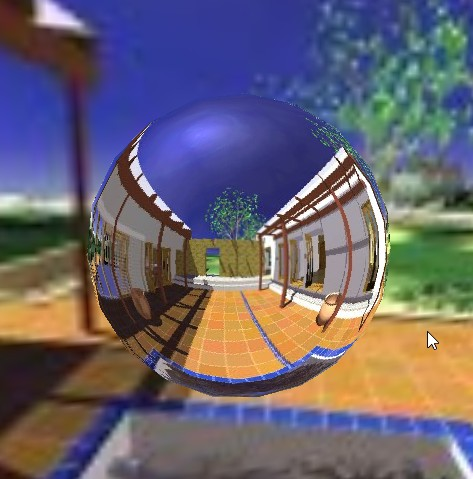
\includegraphics[width=.65\textwidth]{figures/exercise_10_1}
	\end{center}
	\vspace{-4.5ex}\caption{Exercise 10 part 1 and 2}
	\label{fig:exercise_10_1} 
\end{figure}

\section{Part 3}
Implementing glass shader following the instructions gave me the result
below.
\begin{figure}[ht!]
	\begin{center}
		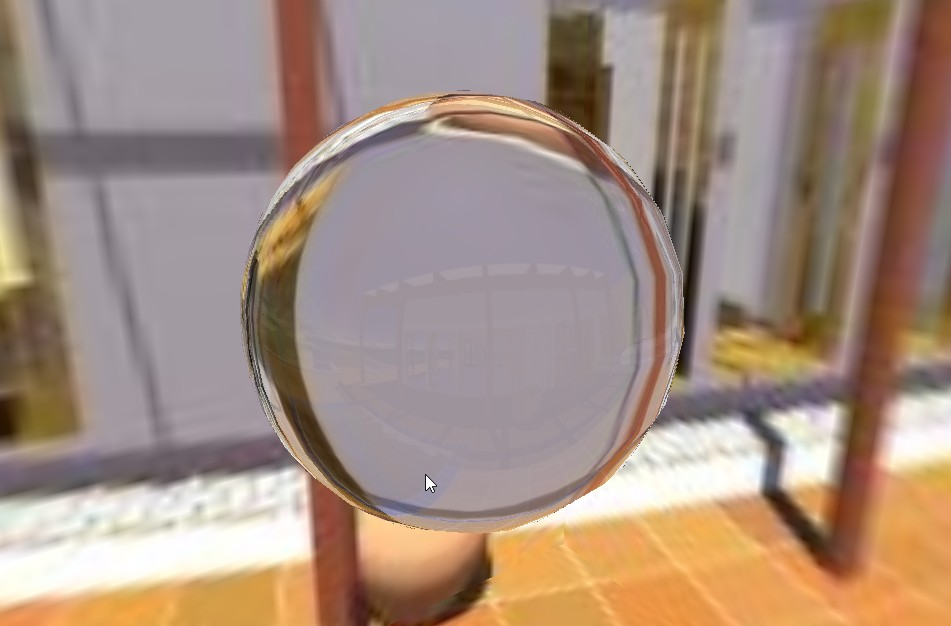
\includegraphics[width=1.0\textwidth]{figures/exercise_10_2}
	\end{center}
	\vspace{-4.5ex}\caption{Exercise 10 part 3}
	\label{fig:exercise_10_2} 
\end{figure}

\section{Part 4 and 5}
Using the following code in fragment shader I managed to get an impression that
the surface is ,,bumpy'' and to add some chromatic dispersion. The intermediate
result of normal vector wrapped around the sphere is shown in the figure \ref{fig:exercise_10_3}.
The results with chromatic dispersion disabled and enabled are shown in figures
\ref{fig:exercise_10_4} and \ref{fig:exercise_10_5} respectively.
\clearpage
\begin{lstlisting}[language=cpp, caption={bump-map fragment shader}]
uniform samplerCube cubemap;
uniform sampler2D textureBump;
uniform vec3 cameraPos;
in vec3 vPosition;
out vec4 fragColor;

vec3 bumpMap(vec3 normal, vec3 position){
	vec3 n = normalize(normal);
	float radius = length(vec3(position));
	float PI = 3.14159265;
	vec2 tangent2 = vec2(acos(position.z/radius), atan(position.y, position.x));
	vec2 tangentUV = vec2(tangent2.x / (2*PI), tangent2.y / PI);
	vec3 T = vec3(cos(tangent2.x)*cos(tangent2.y), cos(tangent2.x)*sin(tangent2.y),-sin(tangent2.x));
	vec3 B = vec3(-sin(tangent2.x)*sin(tangent2.y), sin(tangent2.x)*cos(tangent2.y), 0.0);
	mat3 tbn = mat3(T,B,n);
	vec3 nn = texture(textureBump,tangentUV).xyz;
	vec3 V = (nn - vec3(0.5, 0.5, 0.5))*2.0;
	return normalize(tbn*V);
}

void main(void){
	vec3 normal = bumpMap(normalize(vPosition), vPosition);
	float air = 1.0;
	float glass = 1.62;
	float eta = air/glass;
	float disp = 0.03;
	vec3 incidence = normalize(vPosition - cameraPos);
	vec4 reflection = texture(cubemap, reflect(incidence, normal));
	vec4 refractionR = texture(cubemap, refract(incidence, normal, eta));
	vec4 refractionG = texture(cubemap, refract(incidence, normal, eta-disp));
	vec4 refractionB = texture(cubemap, refract(incidence, normal, eta-(2*disp)));
	vec4 refraction = vec4(refractionR.x, refractionG.y, refractionB.z, 1.0);
	float cosFi = max(dot(normal, -incidence), 0.0);
	float R0 = pow((air - glass) / (air + glass), 2.0);
	float R = R0 + (1.0 - R0)*pow(1.0 - cosFi, 5.0);
	fragColor = R * reflection + (1 - R) * refraction;
}
\end{lstlisting}
\clearpage
\begin{figure}[ht!]
	\begin{center}
		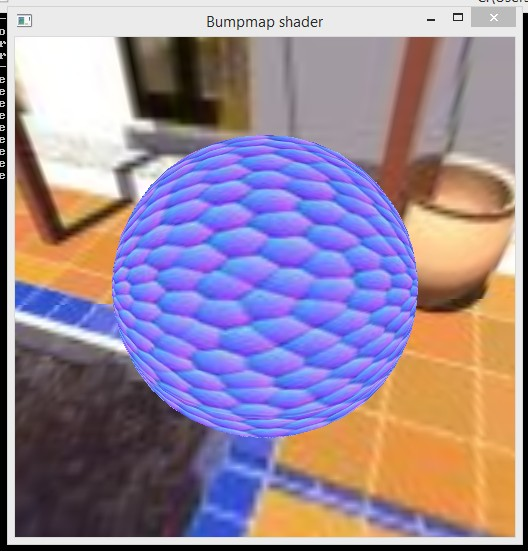
\includegraphics[width=.6\textwidth]{figures/exercise_10_3}
	\end{center}
	\vspace{-4.5ex}\caption{Exercise 10 part 4 intermediate}
	\label{fig:exercise_10_3} 
\end{figure}

\begin{figure}[ht!]
	\begin{center}
		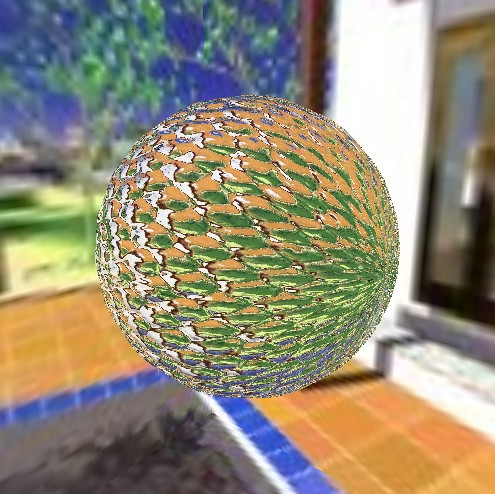
\includegraphics[width=.6\textwidth]{figures/exercise_10_4}
	\end{center}
	\vspace{-4.5ex}\caption{Exercise 10 part 4}
	\label{fig:exercise_10_4} 
\end{figure}

\begin{figure}[ht!]
	\begin{center}
		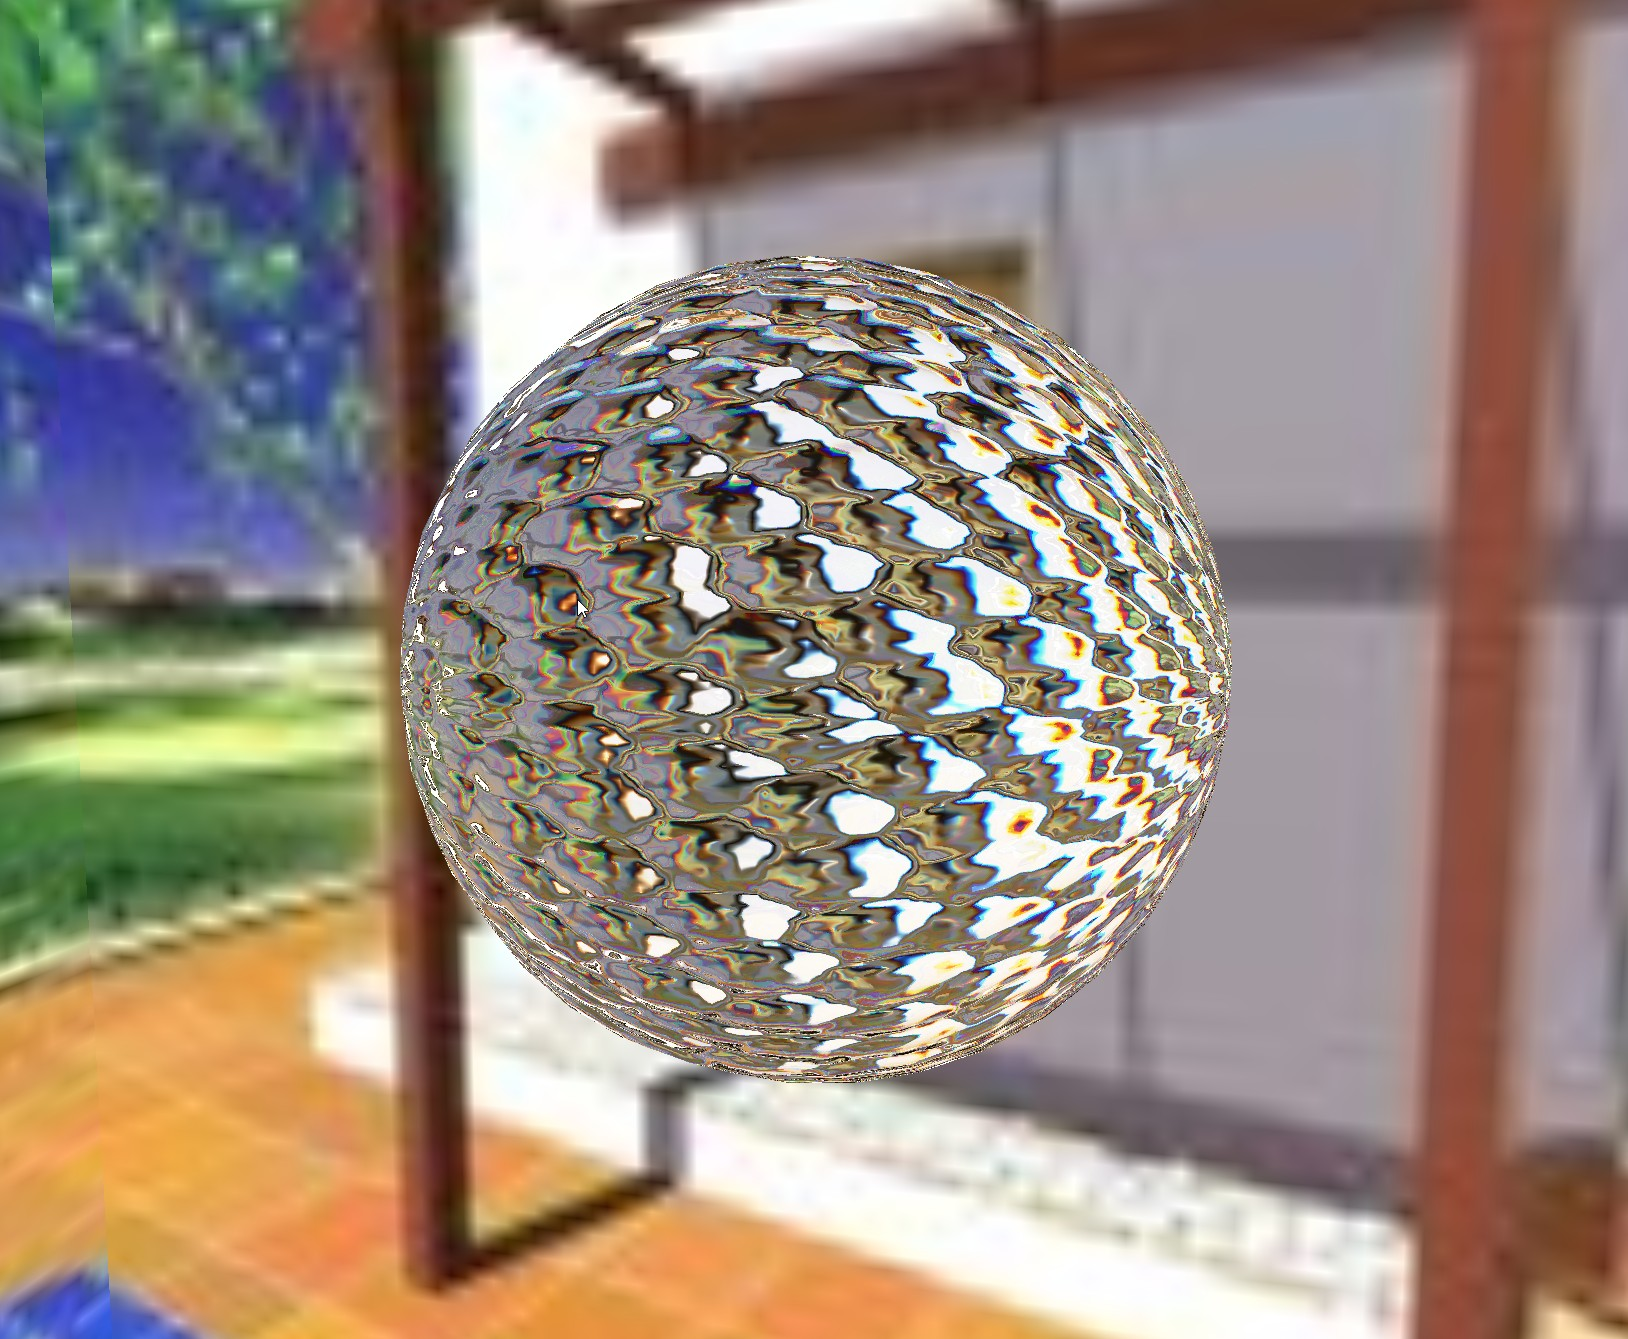
\includegraphics[width=1.0\textwidth]{figures/exercise_10_5}
	\end{center}
	\vspace{-4.5ex}\caption{Exercise 10 part 5}
	\label{fig:exercise_10_5} 
\end{figure}